% !TEX encoding = UTF-8 Unicode
% !TeX spellcheck = en_US


% Latex-Template für die VDI Mechatroniktagung 2015
% Lehrstuhl für Regelungssystemtechnik, TU Dortmund
% Letzte Änderung: 18.02.2014

\documentclass[fleqn,a4paper,10pt]{article}

% Packages
\usepackage{mathptmx} % Times Schriftart (auch in der Math-Umgebung)
\usepackage[german, english]{babel}
\usepackage[utf8]{inputenc} % Deutsche Sonderzeichen/Umlaute gestatten
\usepackage[T1]{fontenc}
\usepackage[nooneline,bf,labelsep=quad,font=small]{caption} % Bildunterschrift linksbündig

\usepackage{multicol}

\usepackage{amsmath} % Zur Abbildung mathematischer Symbole und Formeln
\usepackage{amssymb}
\newcommand{\bm}[1]{\mathbf{#1}}
\renewcommand{\Phi}[1]{\varPhi{#1}}
\newcommand{\rotmat}[2]{{{ }^{#1}\bm{R}}_{#2}}
\newcommand{\ortvek}[4]{{ }_{(#1)}{\bm{#2}}^{#3}_{#4} }
\newcommand{\transp}[0]{{\mathrm{T}}}
\newcommand{\ks}[1]{{(\mathrm{CS})}_{#1}}
\usepackage[fleqn]{nccmath} % Ausrichtung von Gleichungen

\usepackage{graphicx}
\usepackage{graphbox}   % allows to add keys to \includegraphics
\graphicspath{{../kurzfassung/Bilder/}}
\usepackage{color}
\usepackage{geometry}

\usepackage{booktabs} % Erweiterte Tabellenumgebung
\usepackage{cite} % Erweitertes Zitiermöglichkeiten

\usepackage{titlesec} % Abstand vor und hinter Abschnittstiteln.

\usepackage{etoolbox} % Scriptsammlung. Z.B. horizontalen Abstand zwischen Literatureintrag und jeweiligem Label verändern.


% Seiteneinstellungen
\geometry{left=2.025cm, right=2cm, top=2.07cm, bottom=2.8cm} % Geringe Änderungen, um mit Word übereinzustimmen.
\parindent0cm
\columnsep5mm
\parskip 0pt   
\pagestyle{empty}                  % Kopf- und Fußzeile entfernen

% Abschnittsüberschriften
\captionsetup[table]{skip=-1.4ex} % Abstand zwischen Tabelle und Tabellenbeschriftung
\captionsetup[figure]{skip=5mm} % Abstand zwischen Bild und Bildunterschrift

% Paper-Titel
\titlespacing*{\section}{0pt}{6pt}{6pt}
\titlespacing*{\subsection}{0pt}{6pt}{6pt}
\titleformat{\section}{\normalfont\Large\bfseries}{\thesection\hskip 1cm}{0pt}{} % Abstand zwischen Titelnummer und Beschriftung.
\titleformat{\subsection}{\normalfont\large\bfseries}{\thesubsection\hskip 0.7cm}{0pt}{}

% Gleichungen
\setlength{\mathindent}{0.5cm} % Abstand von Gleichungen zum linken Rand.

% Tabelleneinstellungen
%\renewcommand{\arraystretch}{9.5} % Abstand zwischen Zeilen in einer Tabelle -> Steht in Vorlage, führt in Formel-Array zu sehr großem Abstand
\setlength{\tabcolsep}{6pt} % Abstand zwischen Spalten in einer Tabelle

% Umgebungsdefinitionen
\newenvironment{mytitle}{\fontsize{16pt}{1.0} \selectfont \bfseries}{\\} 
\newenvironment*{myabstract}{\begin{Large}\bfseries}{\end{Large}\\[6pt]}%

\renewenvironment{figure}
  {\par\vspace{6pt}\noindent\minipage{\linewidth}}
  {\endminipage\par\vspace{6pt}}


\renewenvironment{table}
  {\par\vspace{6pt}\noindent\minipage{\linewidth}\fontsize{8.5pt}{1.2} \selectfont}
  {\endminipage\par\vspace{6pt}}

\makeatletter

\g@addto@macro\normalsize{%        % Abstand vor und hinter Gleichungsumgebungen.
  \setlength\abovedisplayskip{6pt}
  \setlength\belowdisplayskip{6pt}
  \setlength\abovedisplayshortskip{6pt}
  \setlength\belowdisplayshortskip{6pt}
}

\makeatother

% Literaturverzeichnis
\patchcmd{\thebibliography}{\advance\leftmargin\labelsep}
  {\advance\leftmargin\labelsep \labelsep=0.4cm}{}{} % Horizontalen Abstand anpassen (etoolbox)
\patchcmd{\thebibliography}{\section*}{\section}{}{} % Abschnittsnummer hinzufügen

\let\OLDthebibliography\thebibliography % Vertikalen Abstand anpassen
\renewcommand\thebibliography[1]{
  \OLDthebibliography{#1}
  \setlength{\parskip}{0pt}
  \setlength{\itemsep}{2pt}
}


\begin{document}

\begin{mytitle}
\foreignlanguage{german}{
Maßsynthese für Parallele Roboter: Einheitliche Kinematik und\\ Dynamik mit vollständigen kinematischen Zwangsbedingungen} \\[6pt] % Falls Zeilenumbruch erforderlich, \\[6pt] anfügen.
Dimensional Synthesis of Parallel Robots: Unified Kinematics and\\ Dynamics using Full Kinematic Constraints
\end{mytitle}

Moritz Schappler, Prof. Dr.-Ing. Tobias Ortmaier, Leibniz Universität Hannover, Institut für Mechatronische Systeme, Appelstraße 11a, 30167 Hannover, Deutschland. Korrespondenz: moritz.schappler@imes.uni-hannover.de.

\vspace{24pt} % Bitte nicht entfernen.

\foreignlanguage{german}{
\begin{myabstract} Kurzfassung \end{myabstract}
Durch systematische Struktursynthese wurden bislang eine Vielzahl unterschiedlicher Parallelkinematiken (PKM) beschrieben. 
Um die passendste Roboterkinematik für eine gegebene Aufgabe zu finden, ist eine effiziente und allgemeingültige Auswahlsystematik erforderlich. 
Für einfache Systeme mit mehrwertigen Gelenken wie die Gough-Stewart-PKM liegen bereits Modellierungs- und Optimierungsverfahren vor. 
Für komplexere Strukturen mit mehr einwertigen Gelenken ist die Auswahl an Verfahren eingeschränkter. 
Der vorliegende Beitrag führt allgemeine Ansätze für die Modellierung der Kinematik und Dynamik zusammen, um eine für die Maßsynthese von PKM besonders effiziente Struktur zu erhalten.}


\vspace{12pt} % Bitte nicht entfernen.


\begin{myabstract} Abstract \end{myabstract}
A variety of different structures for parallel kinematic machines (PKM) have been found by means of systematic structural synthesis.
To find the structure that is suited best for a specific task an efficient and generic selection method is necessary.
For simple structures with multi-degree-of-freedom joints like the Gough-Stewart-robot methods for modeling and dimensional optimization are well established.
For more complex structures with single-degree-of-freedom joints less methods are available.
This contribution combines general approaches for the modeling of the kinematics and dynamics of parallel robots to obtain an especially efficient structure for the dimensional synthesis of PKM.

\vspace{18pt} % Bitte nicht entfernen.


\begin{multicols}{2}

\section{Introduction}

\begin{itemize}
\item Die Struktursynthese paralleler Roboter hat durch die systematische Nutzung der Schraubentheorie \cite{KongGos2007} und der evolutionären Morphologie \cite{Gogu2008} eine Vielzahl neuer Parallelkinematiken hervorgebracht, für die Großteils noch keine praktische Anwendung gefunden wurde.
\item Um für gegebene Anforderungen an einen Roboter den bestgeeignetsten auszuwählen, ist eine automatische Auslegung (Maßsynthese) notwendig, die für die Vielzahl verfügbarer Kinematiken anwendbar ist.
\item Der vorliegende Beitrag behandelt eine allgemeine Methodik für die Maßsynthese paralleler Kinematiken unter Ausnutzung struktureller Eigenschaften von Kinematik und Dynamik sowie der effizienten Strukturierung des Optimierungsproblems.
\item Maßsynthese paralleler Roboter großer Schwerpunkt in den 2000er Jahren [Quellen]
\item Bisher hauptsächlich Fokus auf Klassischen PKM mit mehrwertigen Gelenken und wenigen Gliedern [Quellen]
\item Keine systematische Berücksichtigung der Schnittkräfte mittels analytischer Modelle, nur mit FEM [Quellen]
\item Ursache ist die voraussichtlich niedrigere Steifigkeit und Kollisionsanfälligkeit von PKM mit mehrgliedrigen Beinketten
\end{itemize}

Quellen (z.B.)
\cite{JamwalHusXie2015}
\cite{Krefft2006}
\cite{CarboneOttCec2007}
\cite{ZhouBaiHan2011}

Einschränkungen Stand der Technik
\begin{itemize}
\item Modellierung häufig nicht generisch sondern an zu optimierenden Roboter angepasst
\item Für PKM mit mehrgliedrigen Beinketten gibt es nicht immer eine analytische Lösung von Kinematik und Dynamik
\item mehrkriterielle Optimierung relativ aufwändig
\end{itemize}

Beiträge des Papers
\begin{itemize}
\item Anwendung der allgemeinen PKM-Modellierung auf nicht-konventionelle PKM
\item Vorschlag einer effizienten Optimierungsstruktur für die Maßsynthese von PKM
\item Beispiele und simulative Validierung des Verfahrens
\end{itemize}

Gliederung
\ref{sec:sysmdl}
\ref{sec:opti}
\ref{sec:results}
\ref{sec:summary}

\section{System Description and Model}
\label{sec:sysmdl}

%\cite{Merlet2006}
%\cite{Gogu2008}
%\cite{BriotKha2015}

\begin{figure}
\graphicspath{{./Bilder/}}
\centering
\input{Bilder/PKM_Kinematik.pdf_tex}
\captionof{figure}{Sketch of the kinematics of a general parallel robot}
\label{fig:PKM_kinematics}
\end{figure}

%\begin{itemize}
%\item Paralleler Roboter mit 6 FG, Plattform-Pose $\bm{x}$, translatorischer und rotatorischer Teil mit Euler-Winkeln
%\item $m$ Beinketten mit den Gelenkwinkeln $\bm{q}_1$, ..., $\bm{q}_m$ jeweils mit allen aktiven und passiven Gelenken inklusive der Koppelgelenke mit der Plattform
%\item Definition Koppelpunkte $A_i$ und $B_i$, Basis $O$ und Plattform $E$
%\item Schließung der kinematischen ZB über Zwangsbedingungen $\bm{\Phi}$ für gesamte PKM
%%\item Lösung des IKP für jede Beinkette einzeln. 
%\end{itemize}


The general parallel robot model subject to the dimensional synthesis in this paper consists of $m$ leg chains with $n_i$ joints each, which support the moving platform with respect to a fixed base.
A sketch of the robot is depicted in Fig.\,\ref{fig:PKM_kinematics} with the necessary coordinate frames (``CS'') for kinematic modeling, including a base frame $\ks{0}$ of the PKM, base frames $\ks{A_i}$ and virtual end effectors $\ks{E_i}$ for the leg chains  that couple with the platform frames $\ks{B_i}$.
The moving platform frame $\ks{P}$ is expressed with the minimal coordinates $\bm{x}$ containing the position $\bm{x}_\mathrm{t}$ and orientation  $\bm{x}_\mathrm{r}$ (in Euler angles).
All joint coordinates $\bm{q}_i$ of the leg chain $i$ are stacked in the vector

\begin{equation}
\bm{q}^\transp=(\bm{q}_{i}^\transp,\cdots,\bm{q}_{m}^\transp) \quad \mathrm{with}  \quad \bm{q}_i^\transp=(q_{i,1},\cdots,q_{i,n_i}).
\end{equation}

This general model extends the formulation in textbooks \cite{Merlet2006,BriotKha2015} by including coordinates of passive and coupling joints to avoid assumptions on the 	solvability of the kinematic equations (``minimal kinematics set'', \cite{Merlet2006}). 
%A set of kinematic constraints $\bm{\Phi}$ is used to close the kinematic loops w

\subsection{Full Kinematic Constraints}
\label{sec:kinematics}
%\cite{SchapplerTapOrt2019c}


%\begin{itemize}
%\item Zunächst werden die Gelenkgrößen $\bm{q},\dot{\bm{q}},\ddot{\bm{q}}$ des Roboters mittels der vollständigen \emph{inversen Kinematik} berechnet (linker Block in Bild\,\ref{fig:details_kindyn}).
%\item Die dafür notwendigen vollständigen kinematischen Zwangsbedingungen (``ZB'') $\bm{\Phi}$ enthalten für jede Beinkette sowohl den Positions-, als auch den in Euler-Winkeln ausgedrückten Orientierungsfehler \cite{SchapplerTapOrt2019c}.
%\item Definition der ZB mit Formeln
%\item Durch Bildung der Gradienten ($\bm{\Phi}_\bm{q}$ und $\bm{\Phi}_\bm{x}$) können mit der vollständigen Jacobi-Matrix $\tilde{\bm{J}}$ neben den aktiven Gelenkkoordinaten $\bm{q}_\mathrm{a}$ auch passive Gelenke und Schnittgelenke der Plattform berechnet werden, die gemeinsam in $\bm{q}$ zusammengefasst sind.
%\end{itemize}

To be able to solve the inverse kinematics problem for all active and passive joint coordinates $\bm{q}$, a full set of kinematic constraints has to be defined.
In the context of dimensional synthesis, a trajectory of the platform pose $\bm{x}(t)$ is given and has to be accomplished by the simulated parallel robot.
These constraints can e.g. be defined as vector loops between two leg chains, as used in \cite{Gogu2008} on velocity level with the advantage of using linear and angular velocities directly.
The formulation of the full kinematic constraints on position level has the advantage of providing a feasible residual for a gradient-based solution of the inverse kinematics problem, as presented by the authors in \cite{SchapplerTapOrt2019c}. 

%able to solve the inverse kinematics problem 
The translational part of the full kinematic constraints can be formulated as the difference of the coupling point position $B_i$ on the platform and the corresponding coupling joint $E_i$ on the leg chain $i$ with

%For a parallel robot with full mobility, three translational

%
\begin{equation}
\bm{\Phi}_{\mathrm{t},i}(\bm{q}_i,\bm{x}) = - \bm{r}_{A_iB_i}(\bm{x}) + \bm{r}_{A_iB_i}(\bm{q}_i),
\label{equ:kinconstrAB}
\end{equation}
%
as established in the state of the art \cite{Merlet2006} and sketched in Fig.\,\ref{fig:PKM_kinematics}.
The minimal form of the kinematic constraints rotational part is calculated with the Euler angles of the rotational difference of the frames $\ks{E_i}$ on the leg chain and $\ks{B_i}$ on the platform, with
%
\begin{align}
\bm{\Phi}_{\mathrm{r},i}(\bm{q}_i,\bm{x})
=
\bm{\phi}_{XYZ}\left(\rotmat{0}{B_i}^\transp (\bm{x}_{\mathrm{r}})\rotmat{0}{E_i}(\bm{q}_i)\right),
\label{equ:Phir_def_i}
\end{align}
%
as elaborated in detail in \cite{SchapplerTapOrt2019c}.
%
The kinematic constraints for the whole robot are then stacked of the terms for the single leg chains with 
%
\begin{equation}
\bm{\Phi}^\transp
=
(\bm{\Phi}_1^\transp,
\cdots,
\bm{\Phi}_m^\transp
)
\quad
\mathrm{and}
\quad
\bm{\Phi}_i^\transp=(
\bm{\Phi}_{\mathrm{t},i}^\transp, \bm{\Phi}_{\mathrm{r},i}^\transp
).
\label{equ:constr_Phi_PKM}
\end{equation}

The full parallel robot inverse Jacobian 
%
\begin{equation}
\tilde{\bm{J}}^{-1}=-\bm{\Phi}_{\bm{q}}^{-1} \bm{\Phi}_{\bm{x}}
\quad \mathrm{with} \quad
\dot{\bm{q}}=\tilde{\bm{J}}^{-1} \dot{\bm{x}}
\label{equ:jacobian}
\end{equation}
%
is obtained by time differentiation of the constraint equation (\ref{equ:constr_Phi_PKM})  and relates the velocities $\dot{\bm{q}}$ of all joints and the platform $\dot{\bm{x}}$.
To extract only velocity of the actuated joints $\dot{\bm{q}}_\mathrm{a}$, the corresponding rows in $\dot{\bm{q}}$ are extracted with the selection matrix $\bm{P}_{\mathrm{a}}$ with
%
\begin{equation}
\bm{J}^{-1}=\bm{P}_{\mathrm{a}} \tilde{\bm{J}}^{-1}
\quad \mathrm{and} \quad
\bm{q}_{\mathrm{a}} = \bm{P}_{\mathrm{a}} \bm{q}
\label{equ:jacobian_actuation}
\end{equation}
%
giving the analytic Jacobian of the parallel robot, which is square for non-redundant robots and subject to investigations known from literature \cite{Merlet2006}.
The joint accelerations can be obtained by differential calculus to
%
\begin{equation}
\ddot{\bm{q}}=\tilde{\bm{J}}^{-1}\ddot{\bm{x}}+\dot{\tilde{\bm{J}}}^{-1}\dot{\bm{x}}.
\label{equ:acceleration_jacobian}
\end{equation}
%
The nonlinear terms $\bm{\Phi}_{\bm{q}}$ and $\bm{\Phi}_{\bm{x}}$ can be partially  calculated in analytic form, as described in \cite{SchapplerTapOrt2019c}.
The inversion of the $36 \times 36$-matrix $\bm{\Phi}_{\bm{q}}$ (in the full-mobility case) should be performed numerically.
The derivatives of the terms required for (\ref{equ:acceleration_jacobian}) can also be calculated symbolically.

For an efficient calculation of the whole trajectory of the platform for time steps $t=k \Delta t$ with $k=1,...,n_t$, the kinematic relation
%
\begin{equation}
\bm{q}_{k+1}=\bm{q}_k+\dot{\bm{q}}_k \Delta t+\frac{1}{2}\ddot{\bm{q}}_k\Delta t^2
\label{equ:IK_initialvalue}
\end{equation}
%
can be used as an initial value for the gradient-based solution of the inverse kinematics problem.

\subsection{Unified Kinematics and Dynamics}
\label{sec:kindyn}

\begin{figure*}
\graphicspath{{./Bilder/}}
\centering
\input{./Bilder/Details_Kin_Dyn.pdf_tex}
\captionof{figure}{Unified calculation of the inverse kinematics and inverse dynamics for application in the dimensional synthesis}
\label{fig:details_kindyn}
\end{figure*}
%, (\ref{equ:invdyn_leg}), (\ref{equ:coupling_wrench_leg}), (\ref{equ:intforce_fromcoupling}),

%Für die Bestimmung des Energieverbrauchs für eine Referenztrajektorie wird ein allgemeingültiger Ansatz für die \emph{inverse Dynamik} beliebiger paralleler Roboter benötigt.
%Das zu diesem Zweck in \cite{AbdellatifHei2009,DoThanhKotHeiOrt2009b} vorgestellte Prinzip der Energieäquivalenz wird dafür erweitert.
%Zunächst erfolgt die Zerlegung des parallelen Roboters in einzelne Subsysteme (Beinketten und Plattform), in deren jeweiligen Minimalkoordinaten (Gelenk- und Plattformkoordinaten) die Dynamik einzeln nach dem \textsc{Lagrange}schen Formalismus aufgestellt wird (vollständige Massenmatrix $\tilde{\bm{M}}$, Coriolis- und Fliehkraftterme $\tilde{\bm{c}}$, Gravitationsterme $\tilde{\bm{g}}$) \cite{DoThanhKotHeiOrt2009b}.
%Anschließend erfolgt die Projektion der Dynamik in die Minimal-/Plattformkoordinaten $\bm{x}$ des Roboters durch Anwendung des \textsc{D'Alembert}schen Prinzips, woraus die Dynamik-Terme $\bm{M},\bm{c},\bm{g}$ bezogen auf die Plattform resultieren \cite{DoThanhKotHeiOrt2009b,AbdellatifHei2009} (siehe mittlerer Block in Bild\,\ref{fig:details_kindyn}).
%Die Jacobi-Matrix $\tilde{\bm{J}}$ aus der inversen Kinematik kann direkt ohne Neuberechnung für die Dynamik-Projektionsmatrix $\tilde{\bm{R}}$ eingesetzt werden.
%Durch die Verwendung rotatorischer Zwangsbedingungen \cite{SchapplerTapOrt2019c} zusätzlich zu den translatorischen Zwangsbedingungen kann die implizite Annahme aus \cite{AbdellatifHei2009} aufgehoben werden, dass die Beinketten räumlicher Parallelkinematiken in Kugelgelenken enden müssen.
%Diese Bedingung wird z.\,B. von einigen der durch Gosselin et al. \cite{KongGos2007} und Gogu et al. \cite{Gogu2008} erzeugten Roboter nicht erfüllt.

To be able to determine the energy consumption of an arbitrary parallel robot for the reference trajectory of the dimensional synthesis, the inverse dynamics is required.
The application of the principle of energy equivalence for parallel robots from \cite{AbdellatifHei2009,DoThanhKotHeiOrt2009b} has to be extended using the full kinematic constraints from the previous section.
The formulation from Abdellatif et al. \cite{AbdellatifHei2009} only applies for parallel robots which can be described solely with translational constraints (\ref{equ:kinconstrAB}), i.e. robots with leg chains containing at most two links and end in spherical joints in the full mobility case.
Some of the the robots resulting from the structural synthesis from Gosselin et al. \cite{KongGos2007} and Gogu et al. \cite{Gogu2008} do not meet this requirement.

Following the approach from Do Thanh et al. \cite{DoThanhKotHeiOrt2009b} the parallel robot is decomposed into the subsystems leg chains and platform.
The inverse dynamics for the subsystems in their respective minimal coordinates $\bm{q}_i$ and $\bm{x}$ can be obtained with standard methods such as the \textsc{Lagrange} equations.
The resulting terms of the explicit dynamics equation can be assembled as the block diagonal of the full inertia matrix $\tilde{\bm{M}}$ and stacked as the full Coriolis and centrifugal forces vector $\tilde{\bm{c}}$ and gravitational forces vector $\tilde{\bm{g}}$.
The implicit form of the dynamics can be assembled as well as
\begin{equation}
\tilde{\tau} = \tilde{\bm{M}} [\bm{q}^\transp, \bm{x}^\transp]^\transp + \tilde{\bm{c}} + \tilde{\bm{g}}.
\label{equ:subsys_implicit_dyn}
\end{equation}

%, can be stacked in $\tilde{\bm{M}}$, $\tilde{\bm{c}}$, $\tilde{\bm{g}}$ and $\tilde{\bm{\tau}}$, $\tilde{\tau}$

By applying the principle of \textsc{D'Alembert}, the dynamics of the subsystems can be projected into the minimal coordinates $\bm{x}$ of the parallel robot, corresponding to the constraint, closed-loop system, yielding
\begin{equation}
\bm{M}=\tilde{\bm{R}}^\transp\tilde{\bm{M}}\tilde{\bm{R}}, \quad
\bm{c}=\tilde{\bm{R}}^\transp (\tilde{\bm{M}}\dot{\tilde{\bm{R}}}\dot{\bm{x}}+\tilde{\bm{c}}),
\label{equ:invdyn_Mc}
\end{equation}
%
\begin{equation}
\bm{g}=\tilde{\bm{R}}^\transp\tilde{\bm{g}} \quad \mathrm{and} \quad 
\bm{\tau}=\tilde{\bm{R}}^\transp\tilde{\bm{\tau}}.
\label{equ:invdyn_gtau}
\end{equation}

The Jacobian matrix from the inverse kinematics step in (\ref{equ:jacobian}) can be used directly to obtain the projection matrix
%
\begin{equation}
\tilde{\bm{R}}^\transp=\left(\tilde{\bm{J}}^{-\transp},\bm{1}\right).
\label{equ:dyn_projection_matrix}
\end{equation}
%
To reduce the computational effort, the implicit form $\bm{\tau}$ of the inverse dynamics in (\ref{equ:invdyn_gtau}) should be used, avoiding the computation of the inertia and Coriolis terms in (\ref{equ:invdyn_Mc}), which are not used in the dimensional synthesis, unless investigations on inertial forces \cite{FrindtKreHes2010} or Eigen frequencies \cite{JamwalHusXie2015} require the inertia matrix $\bm{M}$.
Further, this allows neglecting the matrix $\dot{\tilde{\bm{J}}}^{-1}$ in (\ref{equ:acceleration_jacobian}), which has low influence on the kinematics.
The actuator force for the calculation of the power consumption of the parallel robot are obtained with the inverse Jacobian from (\ref{equ:jacobian_actuation}) to

\begin{equation}
\bm{\tau}_\mathrm{a}
=\bm{J}^{-\transp} (\bm{M}\ddot{\bm{x}}+\bm{c}+\bm{g})
=\bm{J}^{-\transp} \bm{\tau}.
\label{equ:actforce}
\end{equation}

Using \textsc{D'Alembert}'s principle (``virtual work''), as proposed in \cite{DoThanhKotHeiOrt2009b} requires the definition of kinematic constraints at the position level, which demands some additional efforts for the orientation \cite{SchapplerTapOrt2019c}.
By defining the constraints on velocity level \cite{Gogu2008}, the calculation of the Jacobian is simplified by being able to use angular velocities and corresponding geometric Jacobians instead of Euler angles and their gradient matrices.
The dynamics are then effectively obtained with \textsc{Jourdain}'s principle (``virtual power''), leading to the same result.

\subsection{Internal Forces in Parallel Robots Legs}
\label{sec:intforce}

For an evaluation of the mechanical stress in the structure of the parallel robots legs, the internal forces and moments have to be known.
The projection-based dynamics does not produce cutting forces, since they do not perform work.
Using the Newton-Euler algorithm would provide these forces, but requires setting up a system of equations, which may be less generic than the projection approach.

The internal forces can be reconstructed by adapting the procedure presented in \cite{KhalilGue2004}.


\begin{figure}
\graphicspath{{./Bilder/}}
\centering
\input{./Bilder/PKM_internal_forces.pdf_tex}
\captionof{figure}{Internal forces in the leg chains of the parallel robot}
\label{fig:PKM_internal_forces}
\end{figure}

With the known joint velocity $\dot{\bm{q}}_i$ and acceleration $\ddot{\bm{q}}_i$ from (\ref{equ:jacobian}) and (\ref{equ:acceleration_jacobian}) for all active and passive joints of the leg chain $i$, the internal forces
%
\begin{equation}
\bm{w}_{i,\mathrm{int}}=\bm{w}_{i,\mathrm{int}}(\bm{q}_i,\dot{\bm{q}}_i,\ddot{\bm{q}}_i)
\label{equ:intforce_leg}
\end{equation} % =\begin{pmatrix}\bm{w}_{i,\mathrm{int},0}^\transp & \cdots & \bm{w}_{i,\mathrm{int},n_i}^\transp\end{pmatrix}^\transp
%
can be computed with the recursive Newton-Euler algorithm for serial link kinematics.
As sketched in Fig.\,\ref{fig:PKM_internal_forces}, the single leg chain $i$ cut open can be regarded as a serial link chain with an external wrench $\bm{w}_{B_i}$ acting at the last joint, giving the dynamics equation
 %
\begin{equation}
\bm{\tau}_i
=\bm{M}_i \ddot{\bm{q}}_i + \bm{c}_i + \bm{g}_i
=\bm{\tau}_{\mathrm{m},i} + \bm{J}_{i}^{\transp} \bm{w}_{B_i}.
\label{equ:invdyn_leg}
\end{equation}
%
The Jacobian $\bm{J}_{i}$ projects the external wrench (from perspective of the cut open leg chain) into the joint space coordinates $\bm{q}_i$ of the leg chain.
By assuming no kinematic redundancy and singularity, the equation can be rewritten to
%
\begin{equation}
\bm{w}_{B_i}=\bm{J}_{i}^{-\transp} (\bm{\tau}_i - \bm{\tau}_{\mathrm{m},i}),
\label{equ:coupling_wrench_leg}
\end{equation}
%
yielding the cut force and moment $\bm{w}_{B_i}$ in the coupling point $B_i$.
The motor torque $\bm{\tau}_{\mathrm{m},i}$ in the leg chain has zeros for passive joints and the corresponding entry $\bm{\tau}_{\mathrm{a},i}$ from (\ref{equ:actforce}).

\begin{equation}
\bm{w}_{i,\mathrm{coupl}}=\bm{J}_{i,\mathrm{full}}^{\transp} \bm{w}_{B_i}
\label{equ:intforce_fromcoupling}
\end{equation}


\begin{equation}
\bm{w}_{i} = -\bm{w}_{i,\mathrm{coupl}} + \bm{w}_{i,\mathrm{int}}
\label{equ:intforce_total}
\end{equation}

\subsection{Energy Consumption}
\label{sec:energy}

Since the energy consumption of the parallel robot for a reference trajectory is a scalar value and is correlated with other criteria such as moved mass and joint speeds, it is a good candidate for an objective function of the dimensional synthesis.
%
It is assumed that all electric drives of the actuated joints can exchange power in a common DC link, which represents a future scenario for improving energy efficiency in industrial applications.
Assuming no losses in conversion, the mechanical power of the single robot actuators can be summed up to the electric DC link power
%
\begin{equation}
P_{\mathrm{link}}=\bm{\tau}_\mathrm{a}^\transp \dot{\bm{q}}_\mathrm{a}.
\label{equ:power_link_mech}
\end{equation}
%
Assuming no energy storage or recovery, the electric power required from the grid results to
%
\begin{equation}
P_{\mathrm{grid}}=\left\{\begin{array}{ll} P_{\mathrm{link}}, & P_{\mathrm{link}}>0 \\0, & \mathrm{otherwise.}\end{array}\right.
\label{equ:power_link_grid}
\end{equation}
%
By integrating the power over the time with
%
\begin{equation}
E_{\mathrm{grid}}=\int{} P_{\mathrm{grid}}
\label{equ:energy_integral}
\end{equation}
%
the energy consumption of the parallel robot in the reference trajectory can be obtained.

\section{Optimization}
\label{sec:opti}

\subsection{Formulation of the Problem}

\subsection{Definition of Parameters}

\subsection{Objective Function}



\begin{equation}
z=f_\mathrm{norm}(E_{\mathrm{Netz}})
\end{equation}

Für die Berechnung der \emph{Energie als Zielfunktion} (rechter Block in Bild\,\ref{fig:details_kindyn}) erfolgt eine Projektion der Dynamik auf die Antriebskräfte $\bm{\tau}_\mathrm{a}$. 
Für die dafür notwendige Jacobi-Matrix $\bm{J}$ müssen lediglich die entsprechenden Spalten aus $\tilde{\bm{J}}$ gewählt werden.
Es wird angenommen, dass alle Antriebe ihre Leistung in einem elektrischen Zwischenkreis austauschen können (resultierend zu $P_\mathrm{Kreis}$), was einem zukünftigen Szenario zur Erhöhung der Energieeffizienz entspricht.
Für die aus dem Netz aufzunehmende Leistung $P_\mathrm{Netz}$ wird die Möglichkeit einer  Rückspeisung ausgeschlossen.
Aus der aufintegrierten Energie $E_\mathrm{Netz}$ wird durch eine Normierung $f_\mathrm{norm}(\cdot)$ (mittels arctan-Funktion) der Zielfunktionswert $z$ gebildet.


\subsection{Constraints}

\subsubsection{Geometric Feasibility}

\subsubsection{Inverse Kinematics of Points and Trajectory}

\subsubsection{Joint Limits: Range, Velocity, Configuration}

Joint range



Joint speed

\begin{equation}
f_{\mathrm{jspeed},k} = \max\limits_{t}(\dot{q}_k(t)) / \dot{q}_{k,\mathrm{max}}
\end{equation}
\begin{equation}
p_{\mathrm{jspeed}} = f_\mathrm{Norm}(\max\limits_{k} f_{\mathrm{jspeed},k}-1)
\end{equation}
\subsubsection{Condition Number of the Jacobian}

\begin{equation}
p_{\mathrm{cond}} = f_\mathrm{Norm}(\mathrm{log}(\max\limits_{t}( \mathrm{cond}(\bm{J}(t))))/k_{\mathrm{cond}})
\end{equation}

\subsubsection{Material Stress from Internal Forces}

\begin{itemize}
\item Schnittkräfte und -momente $\bm{w}_{i}$ werden benutzt, um Materialspannung $\sigma_ij$ für alle Segmente $j$ der Beinkette zu berechnen
\item Modell: Hohlzylinder
\end{itemize}

\begin{equation}
f_\mathrm{stress} = \max\limits_{i,j} \frac{\sigma_{i,j}}{\sigma_{i,j,\mathrm{max}}} % \max\limits_{i \in \{1,..m\}} \max\limits_{j \in \{1,..n_i\}}
\end{equation}

\begin{equation}
p_{\mathrm{stress}} = f_\mathrm{Norm}(f_\mathrm{stress}-1)
\end{equation}

\section{Simulation Results}
\label{sec:results}

Erste Ergebnisse der Methodik sind beispielhaft in Bild\,\ref{fig:ergebnisse} dargestellt.
Es wurde eine Optimierung der 6\underline{P}RRS- und  6\underline{R}RRS-Kinematik durchgeführt, wobei das Kugelgelenk (S) einmal beibehalten und einmal durch drei versetzt angeordnete Drehgelenke (RRR) ersetzt wurde, um die allgemeinere Dynamik-Modellierung in der Maßsynthese zu validieren.
Die der Optimierung zugrunde liegende Aufgabe ist das Abfahren der Eckpunkte eines Würfels mit Kantenlänge $30\,\textrm{mm}$ und Kippwinkeln bis zu $10^\circ$ mit einem Beschleunigungs-Trapez-Profil mit einer Gesamt-Verfahrdauer von ca. $11\,\textrm{s}$.

\begin{figure*}
	\centering
	\input{../kurzfassung/Bilder/Optimierung_Ergebnisse.pdf_tex}
	\captionof{figure}{Ergebnisse der Maßsynthese für vier Beispiel-PKM mit Angabe der Zielfunktion $E_\mathrm{Netz}$ und der Parameteranzahl $\mathrm{dim}(\bm{p})$.}
	\label{fig:ergebnisse}
\end{figure*}

%Durch die Vorgabe einer maximalen Plattform-Geschwindigkeit von $1\,\textrm{m/s}$ bzw. $60^\circ\textrm{/s}$ und -Beschleunigung von $3\,\textrm{m/s}^2$ bzw. $180^\circ\textrm{/s}^2$ und einer Zusatzmasse von $3\,\textrm{kg}$ wird versucht, einen ausreichend großen Einfluss der Dynamik auf das Optimierungsergebnis zu erzielen.
Die Optimierungsparameter der durchgeführten Maßsynthese sind u.\,a. die Größenskalierung des Roboters, die \textsc{Denavit-Hartenberg}-Parameter der seriellen Beinketten, die Durchmesser von Gestell und Plattform und Morphologieparameter wie Koppelpunktpaarabstand und Neigung des gestellnahen Gelenks.
%Über die Modellierung der Beinsegmente als Hohlzylinder und der Plattform als Kreisscheibe führt die Veränderung der kinematikbeeinflussenden Parameter
%Parameter wie Gelenk- und Antriebsauswahl, Stärke von Beinsegmenten und Plattform wurden nicht optimiert sondern in späteren Untersuchungen als Entwurfsoptimierung separat betrachtet.
%Einfluss auf die Ergebnisse hatten daher nur die Modellierung der Beinsegmente als Hohlzylinder und der Plattform als Kreisscheibe.
Der PSO-Algorithmus wurde mit 30 Generationen und 70 Individuen parametriert, was angesichts der 15 bis 19 Optimierungsparameter noch gering erscheint.
Der hohen Dimensionalität wurde durch eine Reduzierung der Abhängigkeiten zwischen Parametern und plausibel gewählten Grenzen begegnet.







\subsection{Scenario}

\subsection{Convergence and Distribution}


\begin{figure}
\graphicspath{{./Bilder/}}
\centering
% Bild so einfügen, dass das folgende Beschriftungsbild darüber liegt
% Beim Einfügen des Histogramm-Bilds in InkScape entstehen Grafikfehler
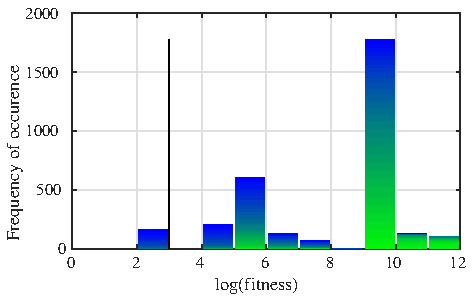
\includegraphics[align=t,smash=br,]{./Bilder/figure_histogram_fitness.pdf}
\input{./Bilder/figure_histogram_fitness_edit.pdf_tex}
\captionof{figure}{Histogram of the fitness function of all particles for one optimization of P6\underline{R}RRS.}
\label{fig:figure_histogram_fitness}
\end{figure}


\subsection{Evaluation of Condition and Material Stress}

\begin{figure}
    \centering
    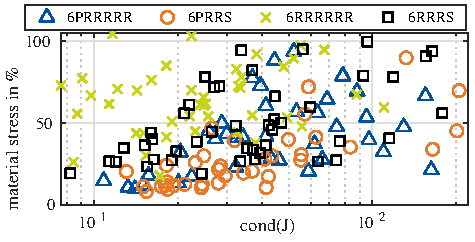
\includegraphics{./Bilder/figure_matstress_vs_condition.pdf}
    \captionof{figure}{Relation of material stress and Jacobian condition number}
    \label{fig:eval_matstress_vs_condition}
\end{figure}



\subsection{Evaluation of Condition and Pivoting Angles}

%Neuer Absatz: Detail zu Optimierung
%\begin{itemize}
%\item Die etablierte Partikel-Schwarm-Optimierung zur Lösung des hochdimensionalen Problems der Parameterfindung von Robotern wird hinsichtlich der Behandlung der Nebenbedingungen modifiziert.
%\item Stückweise definierte Fitness-Funktion mit Zielfunktion und Nebenbedingungen als Strafterm hierarchisch, um Rechenzeit zu sparen. Siehe Bild\,\ref{fig:uebersicht}.
%\item Energieverbrauch als Zielfunktion, da skalare Größe gut vergleichbar und andere Zielfunktionen wie Gesamtmasse und damit Dynamik dazu korrelierend
%\end{itemize}
Für das hochdimensionale Problem der Parameterfindung der Roboter wird die etablierte Partikel-Schwarm-Optimierung (PSO) eingesetzt, wie in Bild\,\ref{fig:uebersicht} skizziert.
Zur effizienten Berücksichtigung von Nebenbedingungen werden diese hierarchisch berechnet und normierte Strafterme $s_i$ direkt in der stückweise definierten Fitness-Funktion $f$ eingesetzt.
Als skalare Zielfunktion $z$ wird der Energieverbrauch des Roboters über eine Referenz-Trajektorie $\bm{x}(t)$ gewählt, was einen direkten Vergleich unterschiedlicher Kinematiken erlaubt.
Des Weiteren wird eine Korrelation mit anderen Zielfunktionen wie Gesamtmasse des Systems oder der Gleichförmigkeit der Eigenschaften (Konditionszahl der Jacobi-Matrix) erwartet.
Die hierarchische Eigenschaft wird durch die Bedingung $s_1(\bm{p})>s_2(\bm{p})>\dots>z(\bm{p})$ und eine Normierung umgesetzt.

\begin{figure*}
	\centering
	\input{../kurzfassung/Bilder/Optimierung_Uebersicht.pdf_tex}
	\captionof{figure}{Überblick über die PSO-Optimierung und die Struktur der Fitness-Funktion mit hierarchischen Nebenbedingungen.}
	\label{fig:uebersicht}
\end{figure*}

%Neuer Absatz: Kinematik und Dynamik
%\begin{itemize}
%\item Generische Ansätze für inverse Dynamik \cite{DoThanhKotHeiOrt2009b,AbdellatifHei2009} bisher explizit nur für klassische PKM definiert, deren Plattform mit Kugelgelenken verbunden ist
%\item Durch Nutzung von vollständigen Zwangsbedingungen (Position und Orientierung) \cite{Gogu2008,SchapplerTapOrt2019c} einheitlicher Ansatz zum Lösen der inversen Kinematik und der inversen Dynamik möglich.
%\item Durch die Reduzierung des Rechenaufwands ist die Auswertung vieler Parameterkombinationen möglich
%\end{itemize}

Zur Bestimmung von Nebenbedingungen wie der Einhaltung der Gelenkwinkelgrenzen ist eine Berechnung der passiven Gelenke und der Plattform-Koppelgelenke notwendig.
%Eine analytische Elimination der passiven Gelenke ist nicht für alle automatisch synthetisierten Strukturen aus möglich.
Zusätzlich wird ein effizienter und allgemeingültiger Ansatz für die Dynamik benötigt.
Der in Bild\,\ref{fig:details_kindyn} dargestellte und im Folgenden skizzierte  Ansatz erfüllt diese Anforderungen.


\section{Summary}
\label{sec:summary}

In dem Konferenzvortrag werden die Ergebnisse und der Ansatz der Optimierung im Detail und weitere Beispiele vorgestellt.
%Dafür wird die Optimierung für weitere Kinematiken und längere Optimierungsdauern durchgeführt sowie statistischen Untersuchungen angestrebt.
Perspektivisch wird auch die Integration der Entwurfsoptimierung von Antriebs- und Segmentdimensionierung und die Behandlung zusätzlicher Nebenbedingungen und Zielfunktionen diskutiert.

%Als weitere Arbeiten sind Plausibilisierungen hinsichtlich Straftermen für Selbstkollisionen und die Reduktion der Optimierungsparameter geplant.

\section{Acknowledgement}

Die Autoren bedanken sich für die Unterstützung durch die Deutsche Forschungsgemeinschaft (DFG, OR 196/33-1).

\bibliographystyle{spmpsci_unsrt}
\bibliography{literatur}

%\clearpage  % Verhindert automatischen Umbruch auf der letzten Seite. Bei Bedarf entfernen.


\end{multicols}


\end{document}